\section{A specific project}\label{sec:A specific project}
%OSS: change the title to getting started? 
\subsubsection*{Motivation} This pattern can help project participants get started, get focused, and make concrete change. It is especially useful for someone who is currently feeling stuck.

\subsubsection*{Context}
%DK This seems like a problem…I would think that the context would be something like "there is an existing shared project with a lot of parts/scope, etc."
We often find ourselves confronted with what seems to be a difficult, complex, or even insurmountable problem. It won't go away, but a workable solution doesn't present itself, either. If there is a candidate solution, it's also clear there are not enough resources for it to be feasible.

\subsubsection*{Forces}~
\begin{tabular}[t]{p{.8\textwidth}@{\hspace{.03\textwidth}}c}
\textbf{Difficulty}: bringing about meaningful change is often hard work. & {\icon \symbol{"0021A2}} \\
\textbf{Inertia}: when things are hard we may feel stuck, wring our hands, or preach to the choir. & 
{\icon \symbol{"00213C}}
\\
\end{tabular}

\subsubsection*{Problem}
We are often blinded by our own prejudices and preferences. Considerable energy goes into pondering, discussing, exploring and feeling stuck. Meanwhile there may be a strong urge to make more concrete progress, and time is passing by. In a group setting, when the forward-movers ultimately try to act, those who are more wrapped up in the experience of pondering and exploring may attempt to shut them down, if they feel that they are being left behind. Inaction may seem like the only safe choice, but it has risks too.

\subsubsection*{Solution} 
One way to make progress when you're stuck is to ask a specific question to someone who may be able to help you get unstuck. Formulating a question helps your thinking become more concrete. Sometimes you'll see that a solution was within your grasp all along.  Sometimes one question won't be enough, but you can repeat the process. In this way, you can reduce a large, complex, or ephemeral concern can be transformed into a collection of smaller, specific, manageable tasks. Use a \patternname{Scrapbook} to make note of all the small things, and weave them into your project \patternname{Roadmap}. This will show how the small pieces relate to the bigger picture. If you have a fairly specific idea about what you want to do, but you're finding it difficult to get it done, don't just ask for advice: recruit material help (cf.~\patternname{Carrying capacity}). One example of a specific project from the Peeragogy project is our work on this paper, which had a specific target audience, a set of associated deadlines, and allowed us to get help from pattern experts. 

% DK: This seems a bit speculative, “If you are able…” What steps does this solution entail? How do you know that a project is sufficiently specific? The front part of the pattern makes it sound like the point of view of the pattern is from someone coming into a project looking for something to do, but is there a piece of this pattern for people on a project with ideas about what to do but without the bandwidth to do it? I.e. someone populating the Roadmap with Specific Projects Is there some risk about being too specific about a project?
\subsubsection*{Rationale} 
We've seen time and again that having a specific project is a recipe for getting concrete, and that getting concrete is necessary for bringing about change. Asking for help (which is what happens when you vocalize a question) is one of the best ways to gain coherence. Making yourself understood can go a long way toward resolving deeper difficulties.

%OSS: Tell a lightning story for your resolution? We talk about questions a lot. Confusing? Avoid question and talk more specifically about projects
\subsubsection*{Resolution}
Where you run into \textbf{difficulty}, getting specific paves the way for incremental forward progress and helps to overcome \textbf{inertia}. The struggle between consensus and action is resolved in a tangible project that combines action with dialog. Learning something new is a strong sign that things are working.
Real change starts out ``bite-sized.'' 
% If you want something to happen, get specific.
%OSS: What does Wikipedia ask?

\subsubsection*{Example 1}
% add link 
At first glance, the Wikimedia Foundation's mission presents an overwhelming concept.\footnote{\url{https://wikimediafoundation.org/wiki/Mission_statement}} Where do we get started on a project with a global scale? How do we organise work?
%%%%
In practice, many future Wikipedians jump in, get to know other Wikipedia users, and start working on a focused todo list in
\patternname{A specific project}.
%%%
Within Wikipedia, these are known as ``WikiProjects.''\footnote{\url{https://en.wikipedia.org/wiki/Wikipedia:WikiProject_Council/Directory}}\textsuperscript{,}\footnote{\url{https://en.wikipedia.org/wiki/Wikipedia:WikiProject_Council/Guide}}
Guidance is available on how to start new WikiProjects.\footnote{\url{https://en.wikipedia.org/wiki/Wikipedia:WikiProject_Council/Guide/WikiProject}}
%%%
The Wikimedia Foundation also runs other public projects, including the Wikipedia Education Program and the GLAM Wiki (for Galleries, Libraries, Archives, and Museums).\footnote{\url{https://outreach.wikimedia.org/wiki/Education/Wikipedia_Education_Collaborative/Tasks}}\textsuperscript{,}\footnote{\url{https://outreach.wikimedia.org/wiki/GLAM}}  The latter maintains a \emph{list of case studies that describes specific projects undertaken by cultural organizations and Wikimedia}.\footnote{\url{https://outreach.wikimedia.org/wiki/GLAM/Case_studies}}

\begin{wrapfigure}{r}{.47\textwidth}
\vspace{-.7cm}
\begin{center}
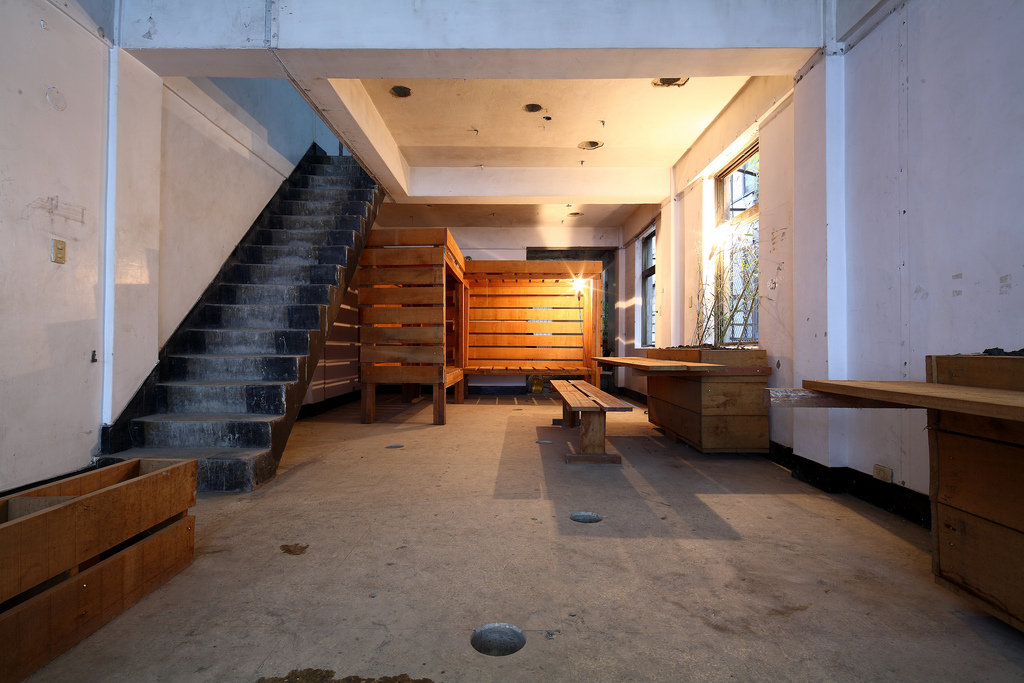
\includegraphics[width=.45\textwidth]{Ruin_Academy_Dorm}
\end{center}
\vspace{-.5cm}
\caption{Ruin Academy Dormitory, Taipei, Taiwan. 
%Public domain.
\label{dormitory}
}
\vspace{-.3cm}
\end{wrapfigure}

%OSS: What example is happening here?
\subsubsection*{Example 2}
%   Between class, studying, tests, papers, exams, friendships, sports, student life, remembering to eat, and more it is easy to get lost and give up.
% life for incoming students can become overwhelming quickly.
At a traditional university,  living together with others, students see that they are not alone in their worries and frustrations. In a peeragogical learning environment, a Dormitory could be seen as an ``optional extra,'' since studying
from where you live is often an option already. Many will have an active social life outside of their peer learning projects.  Even so, a short-term rental or a time-shared cooperatively-owned living\slash working space may be an asset for peeragogues who need to get together to work on \patternname{A specific project}.

% \subsubsection*{Summary}
% ``''

\begin{framed}
\noindent 
\emph{What's Next in the Peeragogy Project}
\definecollection{SpecificWN}
\begin{collectinmacro}{\SpecificWN}{}{}
We need to build specific, tangible ``what's next'' steps and carry them out with concrete actions. 
\end{collectinmacro}
\SpecificWN
\end{framed}

